%
% waerme.tex
%
% (c) 2020 Prof Dr Andreas Müller, Hochschule Rapperswil
%
\begin{frame}
\frametitle{Vergleich numerische Lösung}
\vspace{-15pt}
\begin{center}
\definecolor{rot}{rgb}{1.0,0.0,0.2}
\definecolor{gruen}{rgb}{0.4,0.8,0.2}
\definecolor{blau}{rgb}{0.2,0.6,1.0}
\begin{tikzpicture}[>=latex,thick]

\uncover<1>{
\node at (0,0) {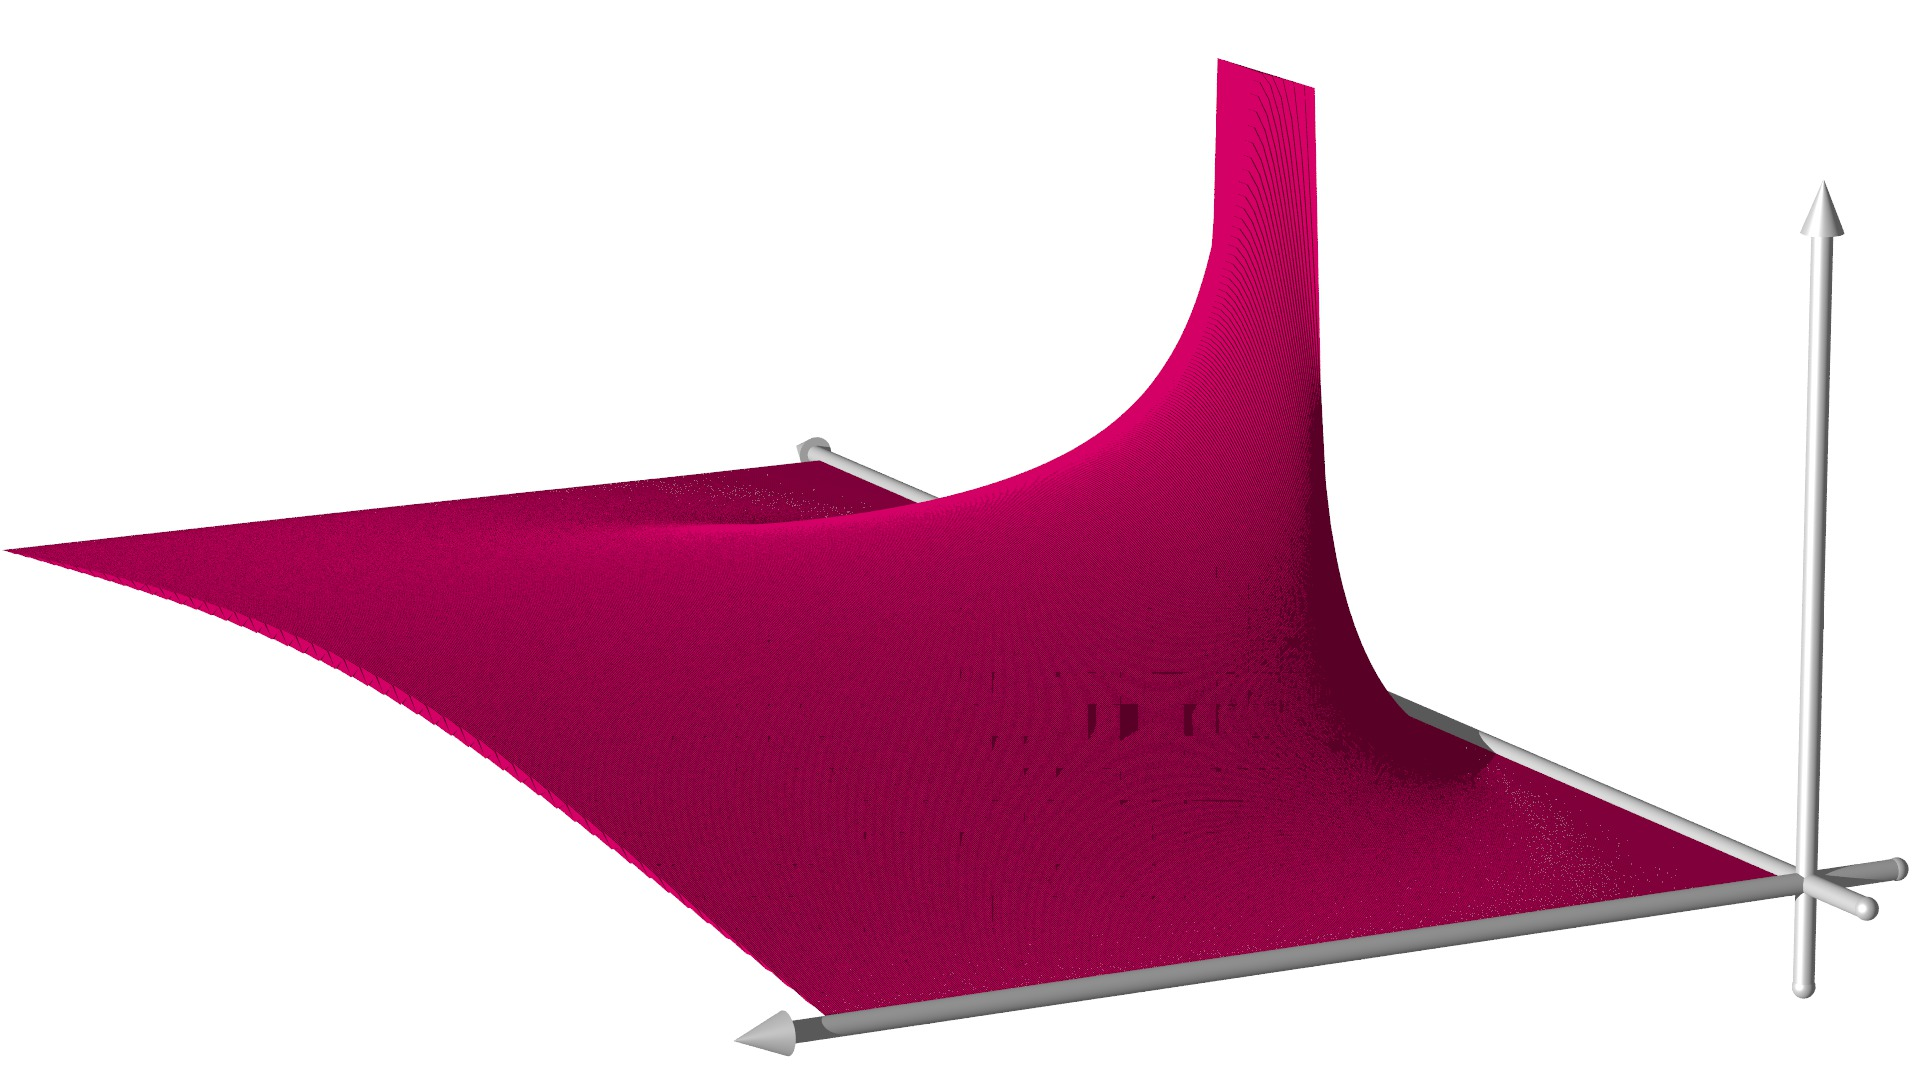
\includegraphics[width=13.4cm]{../slides/8/explizit.jpg}};
}
\uncover<2>{
\node at (0,0) {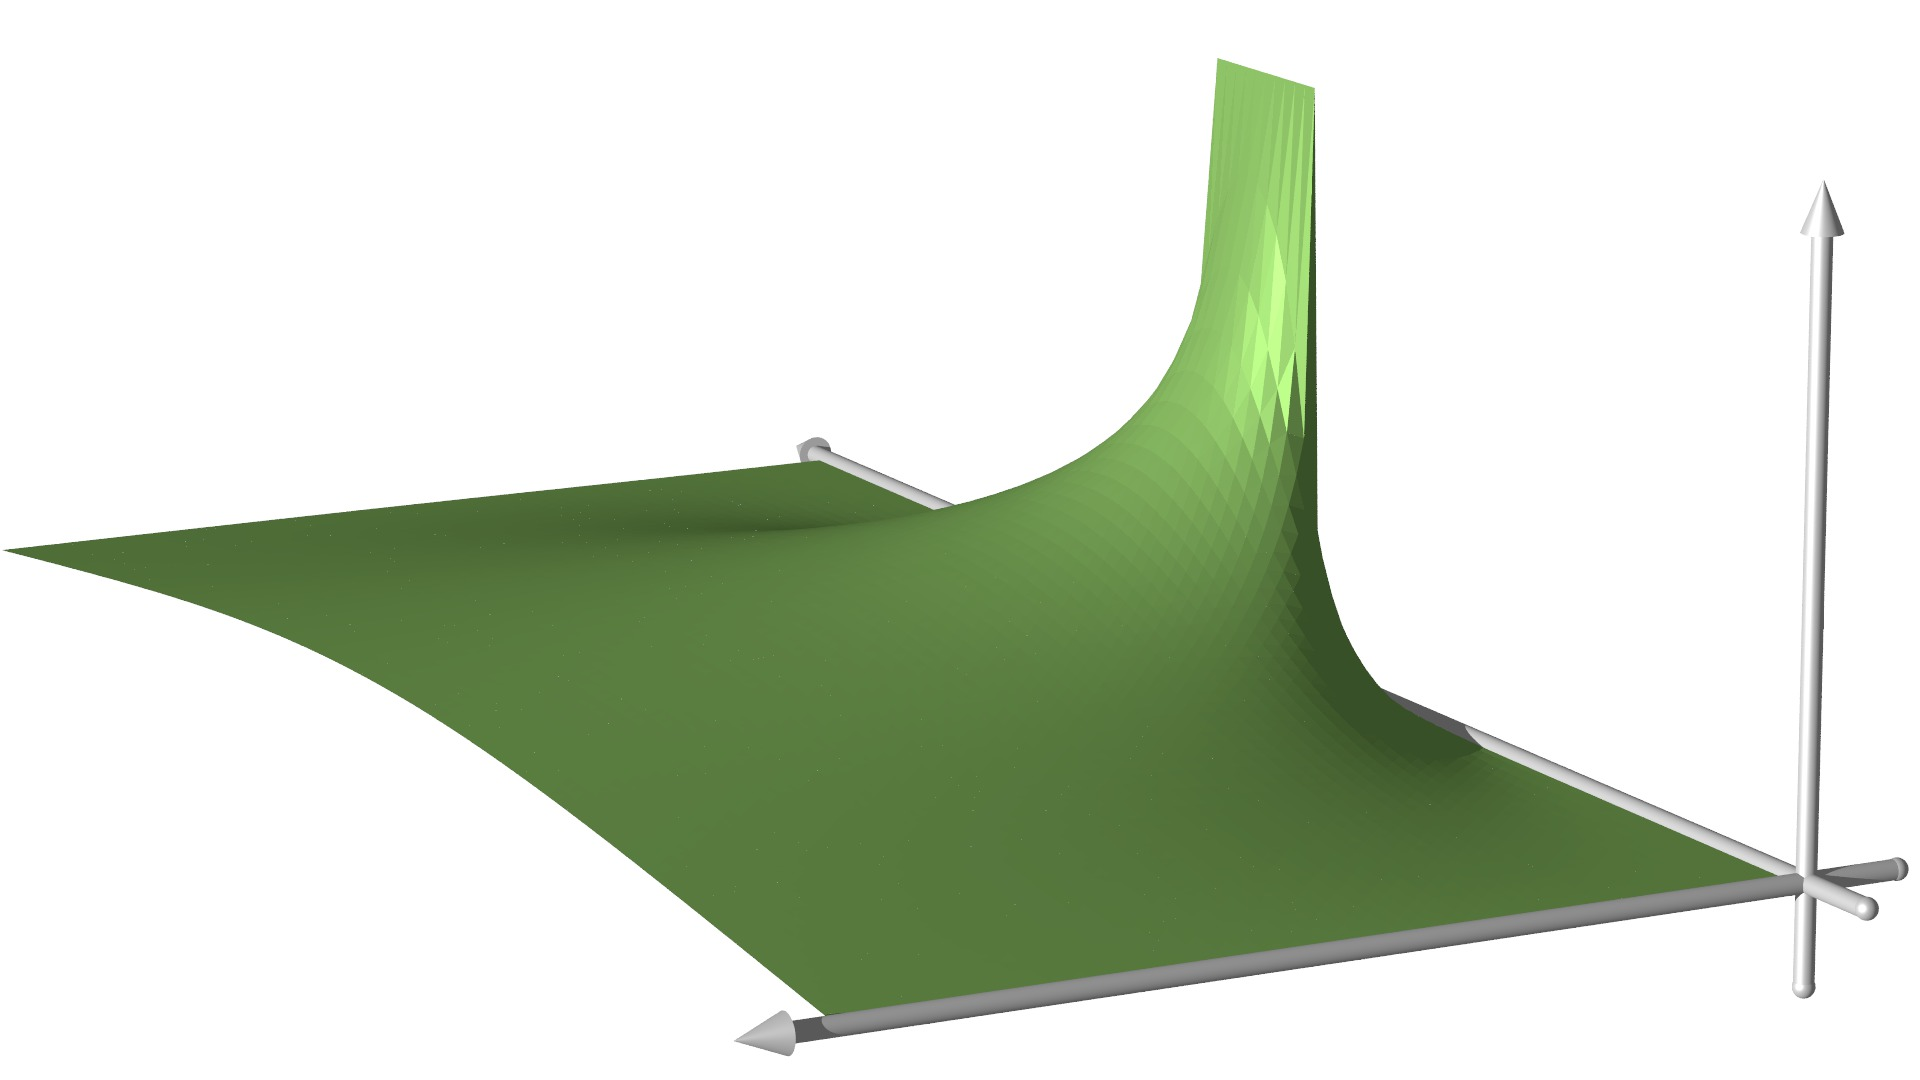
\includegraphics[width=13.4cm]{../slides/8/implizit.jpg}};
}
\uncover<3>{
\node at (0,0) {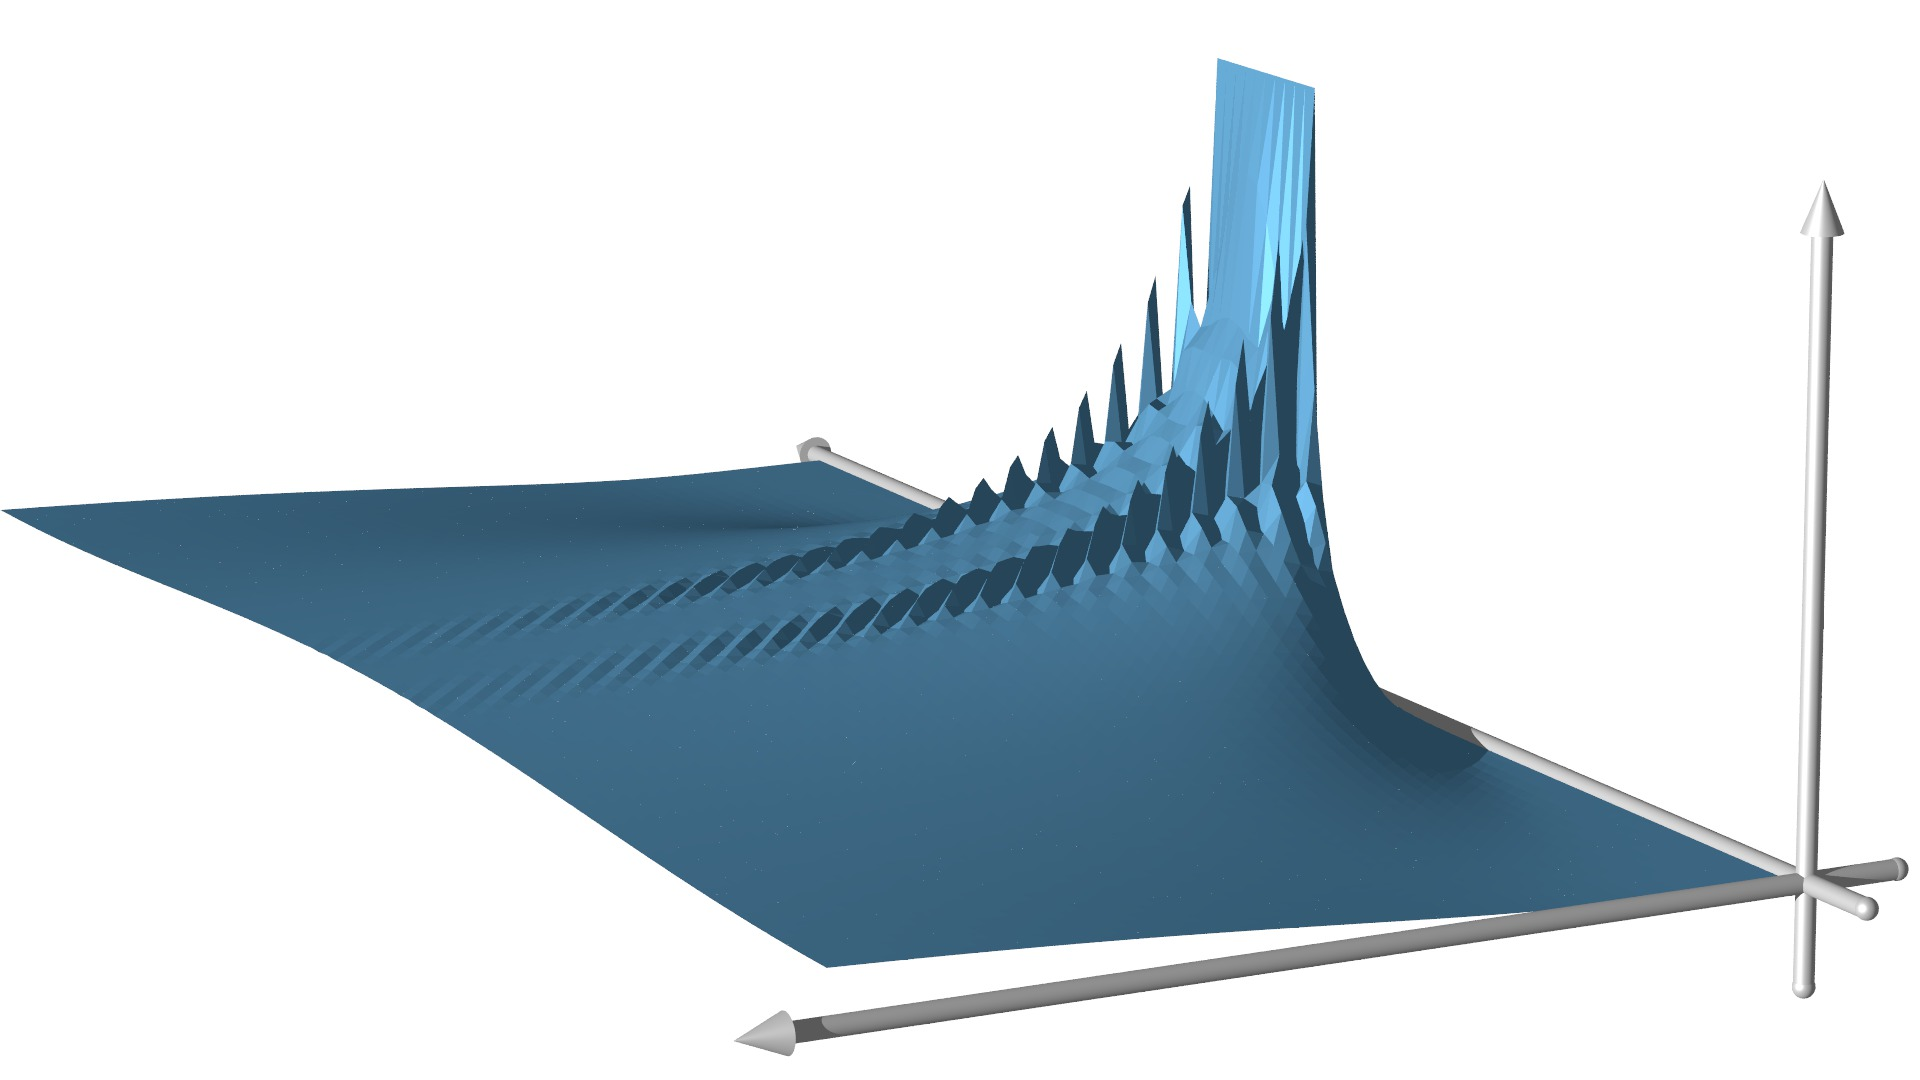
\includegraphics[width=13.4cm]{../slides/8/cranknicholson.jpg}};
}
\uncover<4>{
\node at (0,0) {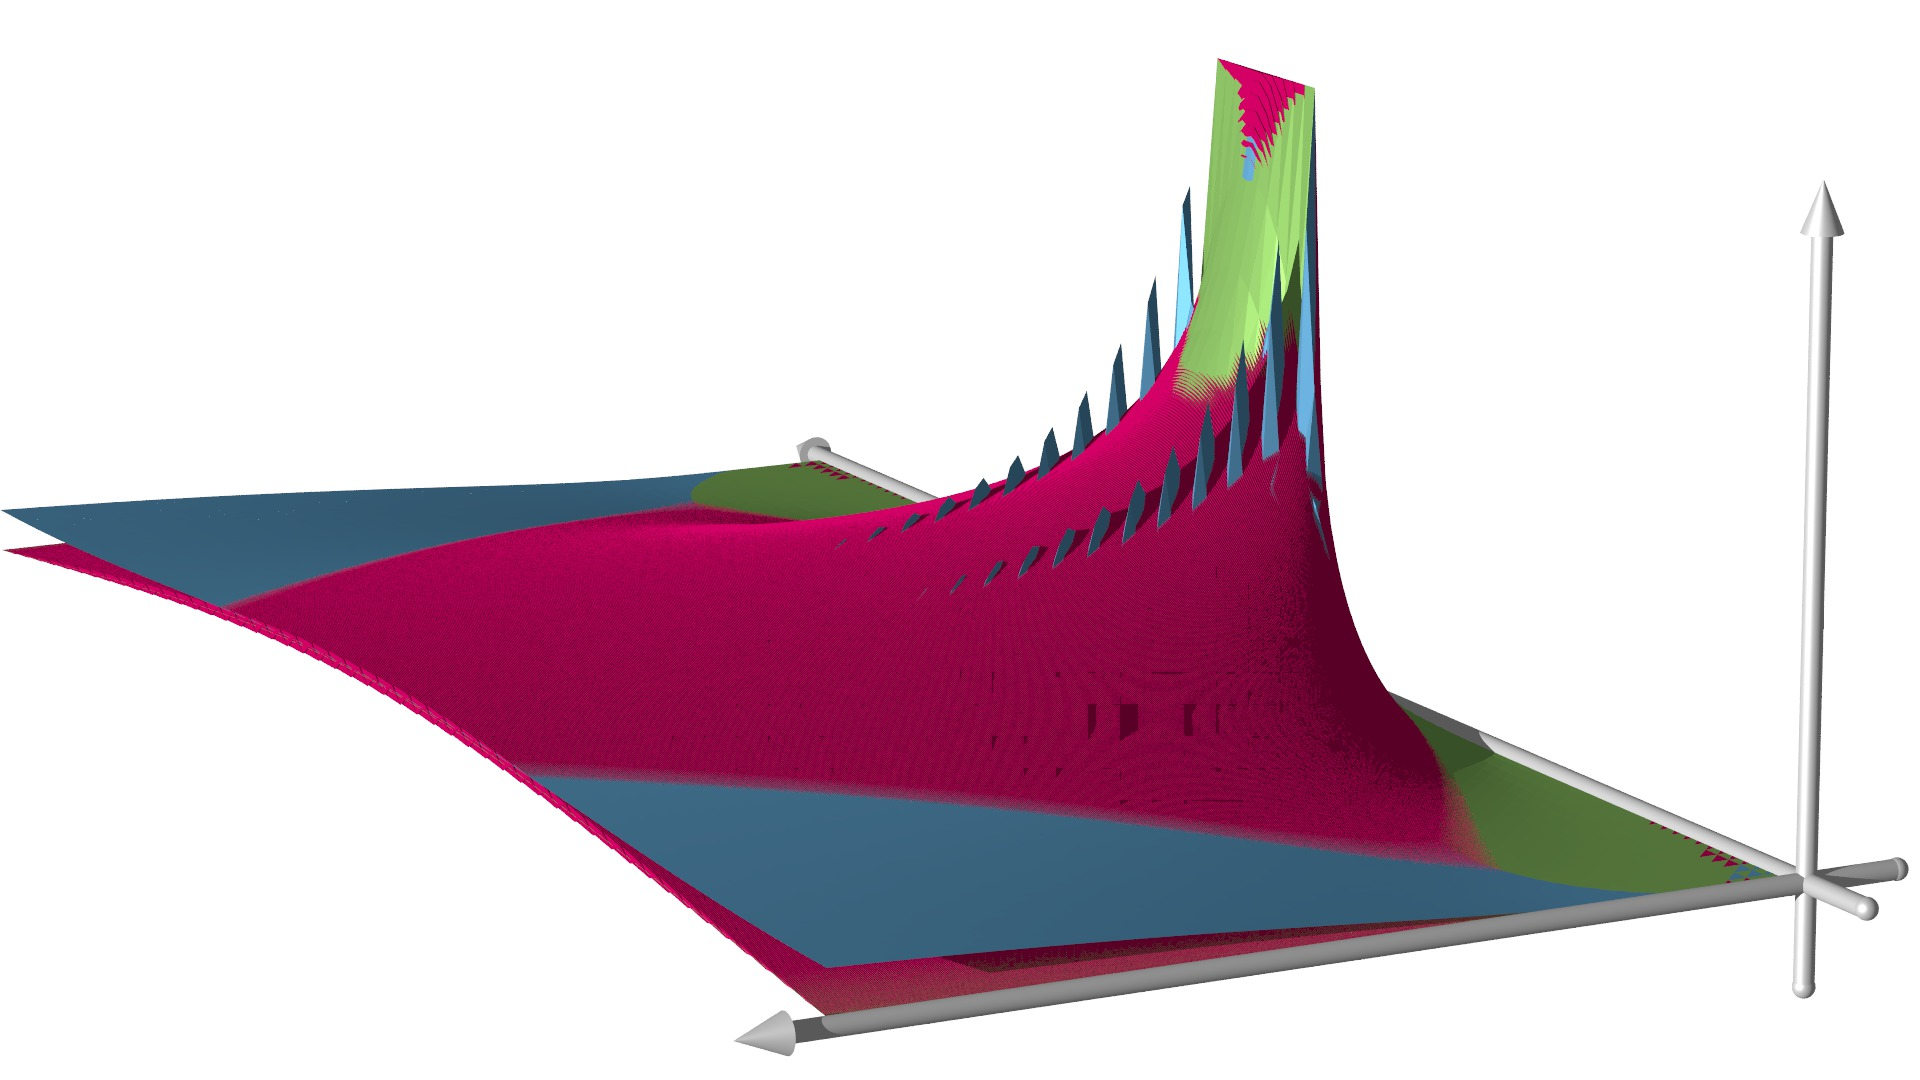
\includegraphics[width=13.4cm]{../slides/8/combined.jpg}};
}

\only<1,4>{
\fill[color=rot] (-6.5,2.85) rectangle (-6.1,3.15);
\node[color=rot]   at (-6,3.0) [right] {Euler vorwärts};
}

\only<2,4>{
\fill[color=gruen] (-6.5,2.05) rectangle (-6.1,2.35);
\node[color=gruen]  at (-6,2.2) [right] {Euler rückwärts};
}

\only<3-4>{
\fill[color=blau] (-6.5,1.25) rectangle (-6.1,1.55);
\node[color=blau] at (-6,1.4) [right] {Crank-Nicholson};
}

\node at (-1.6,-3.2) {$t$};
\node at (-1,0.9) {$x$};
\node at (6.2,2.7) {$u$};
\end{tikzpicture}
\end{center}
\end{frame}
